\begin{figure}[t]
	\centering
	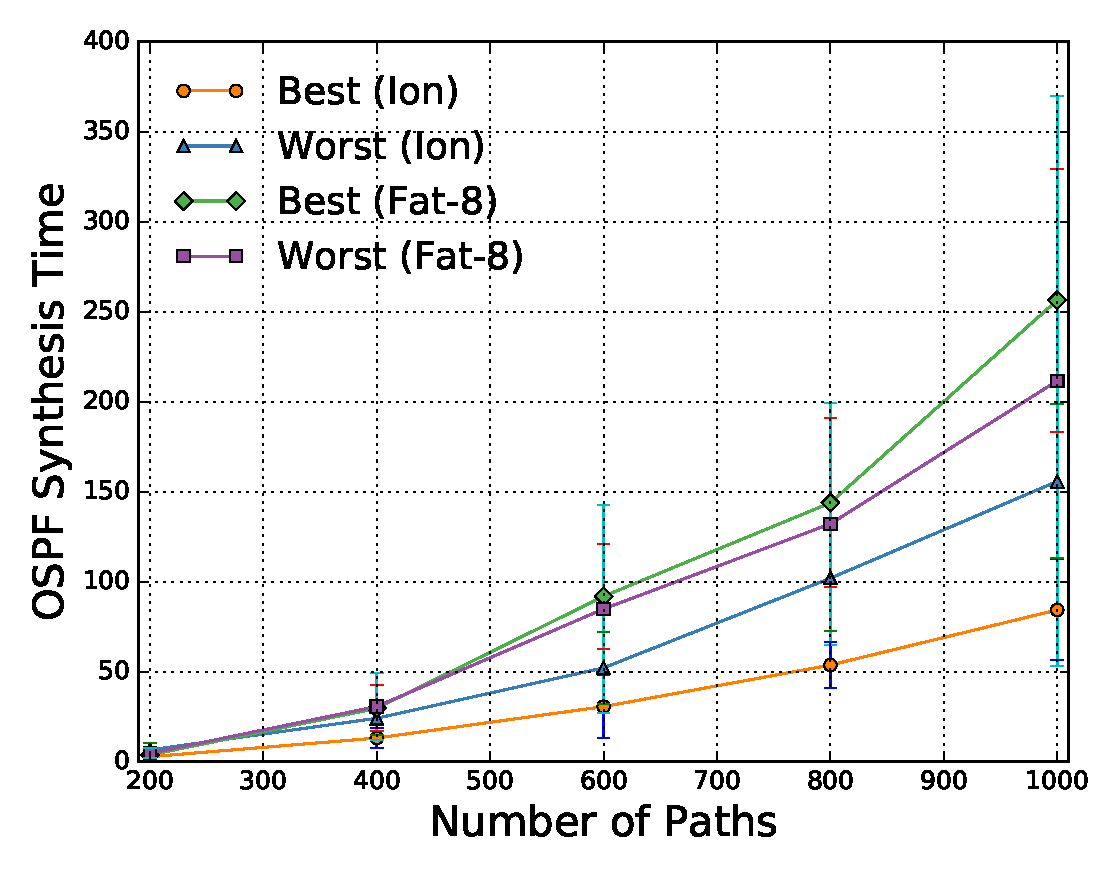
\includegraphics[width=0.7\columnwidth]{figures/ospfSynthesisTimeMCMC.eps}
	\compactcaption{MCMC OSPF Synthesis time}
	\label{fig:ospfmcmc}
\end{figure}


\begin{figure}[t]
	\centering
	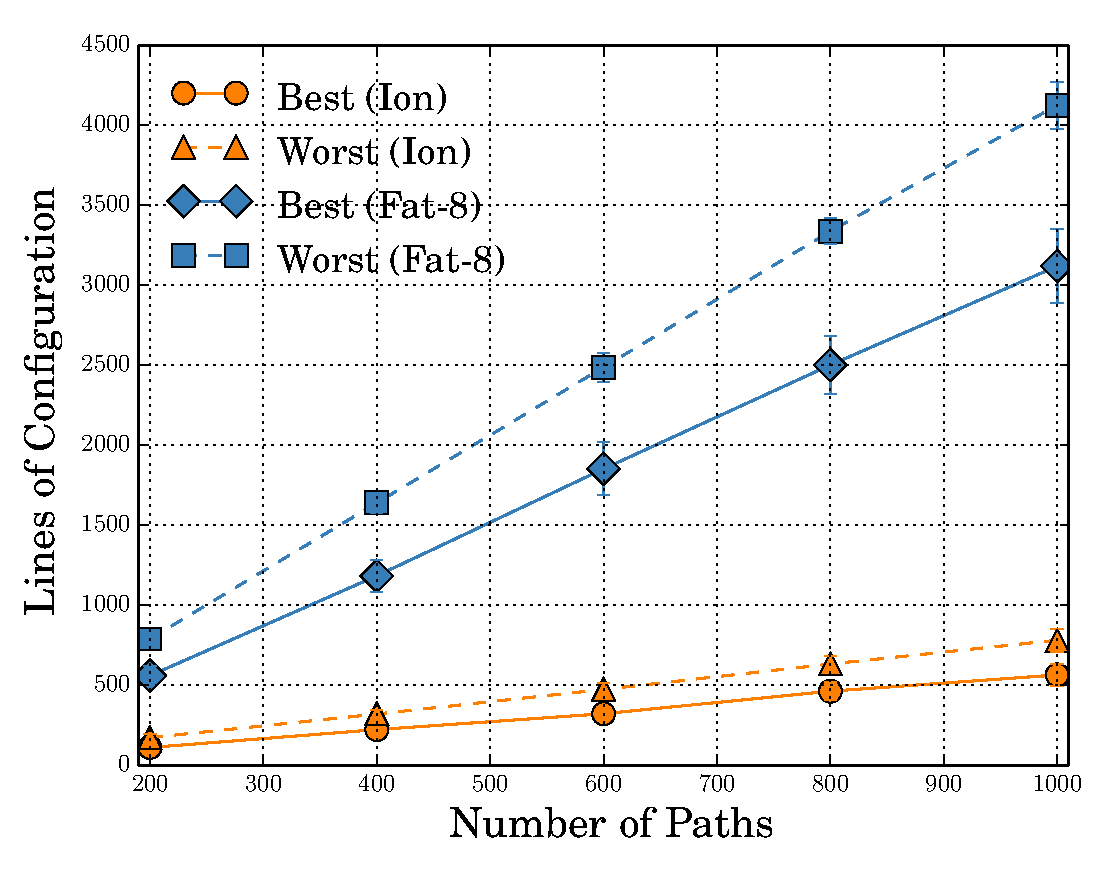
\includegraphics[width=0.7\columnwidth]{figures/confMCMC.eps}
	\compactcaption{MCMC Lines of Conf}
	\label{fig:confmcmc}
\end{figure}

\begin{figure}[t]
	\centering
	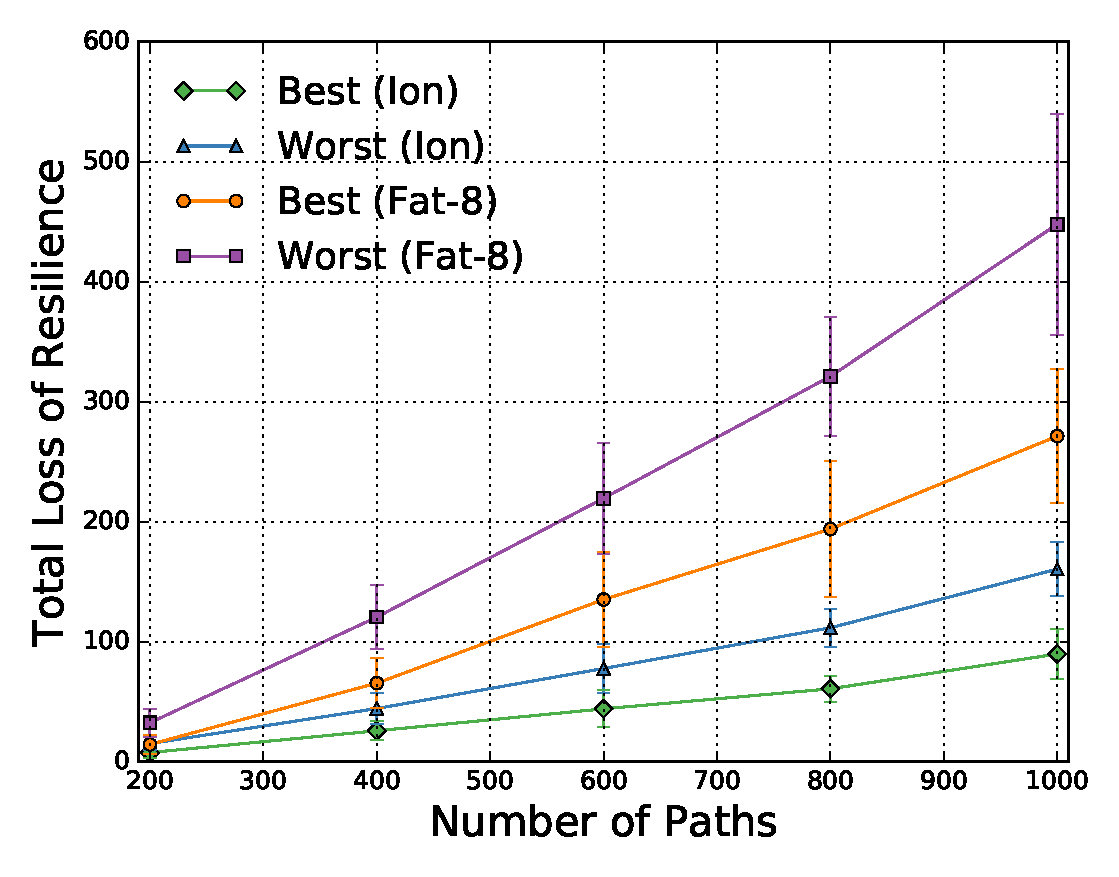
\includegraphics[width=0.7\columnwidth]{figures/TRLMCMC.eps}
	\compactcaption{MCMC TRL}
	\label{fig:trlmcmc}
\end{figure}

\begin{figure}[t]
	\centering
	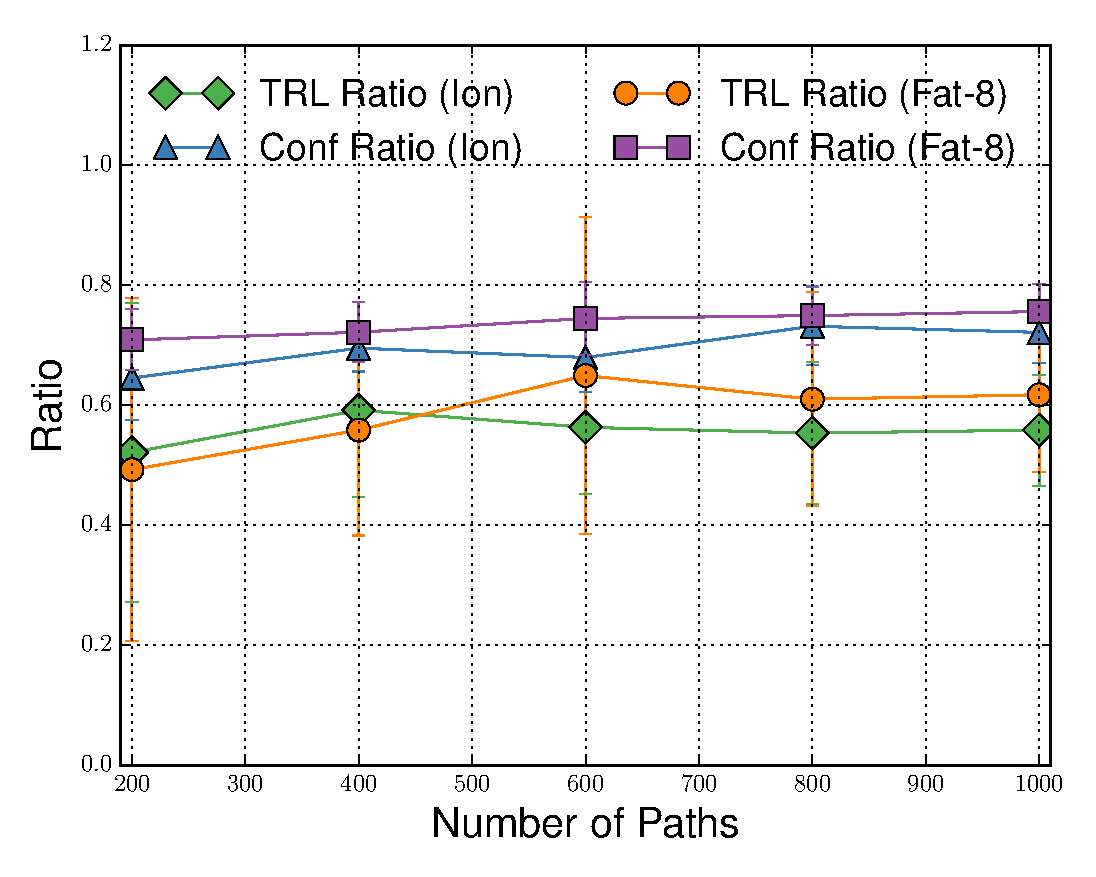
\includegraphics[width=0.7\columnwidth]{figures/ratioMCMC.eps}
	\compactcaption{MCMC Ratios}
	\label{fig:ratiomcmc}
\end{figure}

\begin{figure}[t]
	\centering
	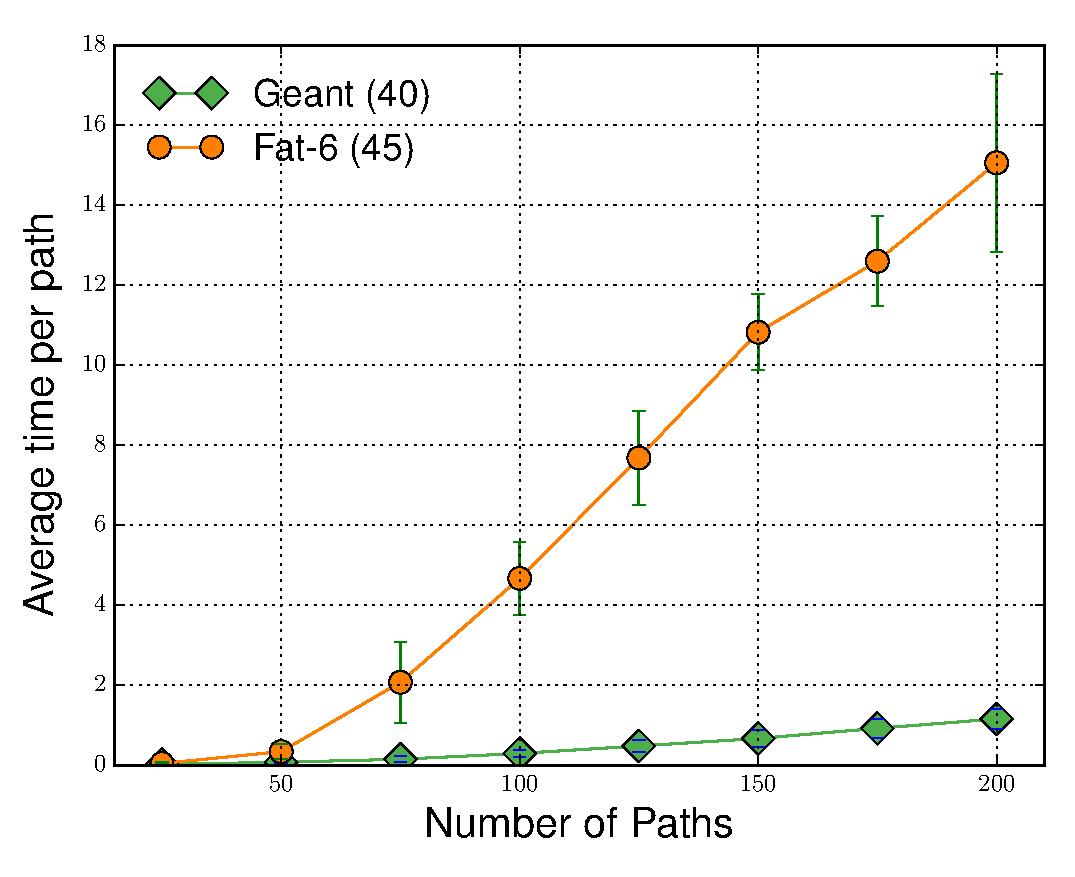
\includegraphics[width=0.7\columnwidth]{figures/ospfTime.eps}
	\compactcaption{OSPF Synthesis Time}
	\label{fig:ospftime}
\end{figure}

\begin{figure}[t]
	\centering
	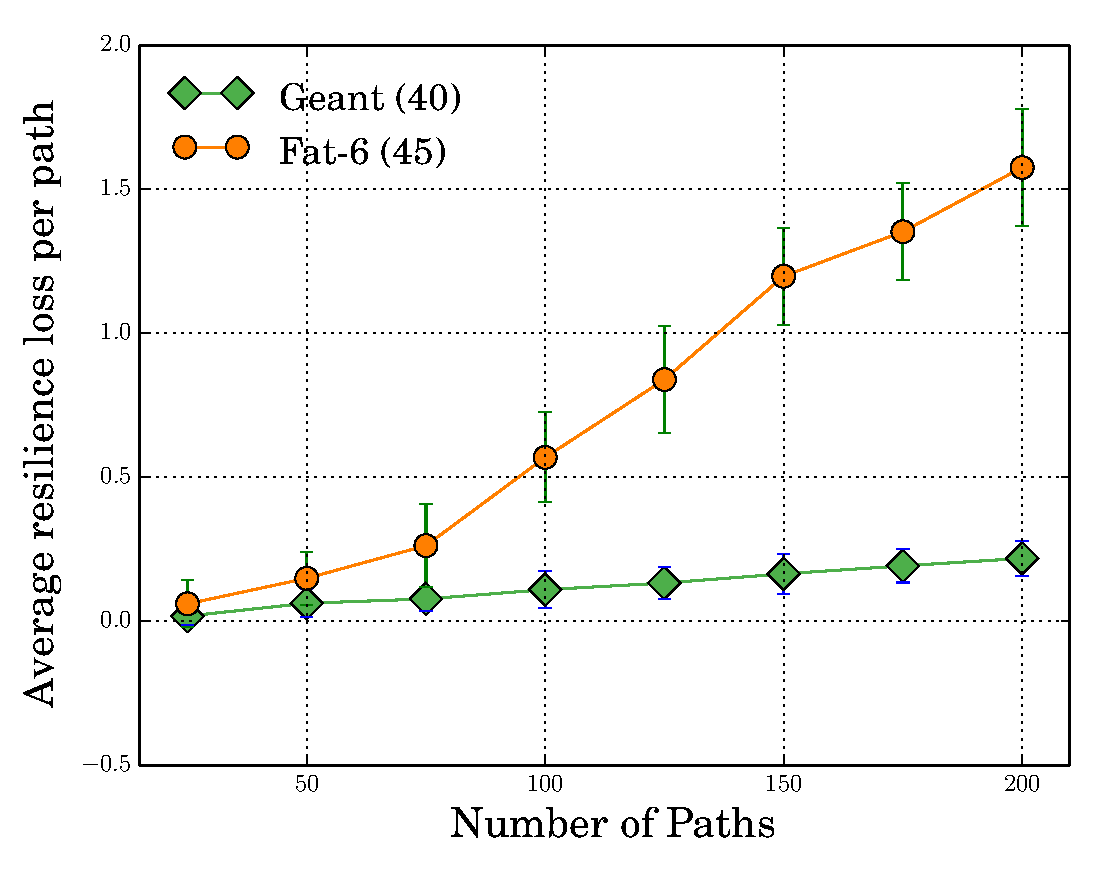
\includegraphics[width=0.7\columnwidth]{figures/ospfTRL.eps}
	\compactcaption{OSPF Loss of Resilience}
	\label{fig:ospfloss}
\end{figure}


\section{Evaluation}
Ion (125 nodes) and Geant(40)

